\documentclass[a4paper, 14pt]{extarticle}
\usepackage[english,russian]{babel}
\usepackage[T1]{fontenc}
\usepackage[utf8]{inputenc}
\usepackage{fontspec}
\usepackage{indentfirst}
\usepackage{enumitem}
\usepackage{graphicx}
\usepackage[
  left=20mm,
  right=10mm,
  top=20mm,
  bottom=20mm
]{geometry}
\usepackage{parskip}
\usepackage{titlesec}
\usepackage{xurl}
\usepackage{hyperref}
\usepackage{float}
\usepackage[
  figurename=Рисунок,
  labelsep=endash,
  justification=centering
]{caption}
\usepackage[outputdir=build, newfloat]{minted}
\usepackage{chngcntr}

\selectlanguage{russian}

\hypersetup{
  colorlinks=true,
  linkcolor=black,
  filecolor=blue,
  urlcolor=blue,
}

\renewcommand*{\labelitemi}{---}
\setmainfont{Times New Roman}
\setmonofont{JetBrains Mono}[
  SizeFeatures={Size=11},
]

\newenvironment{code}{\captionsetup{type=figure}}{}
\BeforeBeginEnvironment{code}{\bigskip}
\AfterEndEnvironment{code}{\bigskip}

\setminted{
  fontsize=\footnotesize,
}

\setlength{\parskip}{6pt}

\setlength{\parindent}{1.25cm}
\setlist[itemize]{itemsep=0em,topsep=0em,parsep=0em,partopsep=0em,leftmargin=2.0cm,wide}
\setlist[enumerate]{itemsep=0em,topsep=0em,parsep=0em,partopsep=0em,leftmargin=2.0cm,wide}

\renewcommand{\thesection}{\indent\arabic{section}.}
\renewcommand{\thesubsection}{\indent\thesection\arabic{subsection}.}
\renewcommand{\thesubsubsection}{\indent\thesubsection\arabic{subsubsection}.}

\titleformat{\section}{\normalfont\bfseries}{\thesection}{0.5em}{}
\titleformat{\subsection}{\normalfont\bfseries}{\thesubsection}{0.5em}{}
\titleformat{\subsubsection}{\normalfont\bfseries}{\thesubsubsection}{0.5em}{}

\titleformat*{\section}{\normalfont\bfseries}
\titleformat*{\subsection}{\normalfont\bfseries}
\titleformat*{\subsubsection}{\normalfont\bfseries}

\titlespacing{\section}{\parindent}{\parskip}{\parskip}
\titlespacing{\subsection}{\parindent}{\parskip}{\parskip}
\titlespacing{\subsubsection}{\parindent}{\parskip}{\parskip}

\begin{document}

\begin{titlepage}
  \vspace{0pt plus2fill}
  \noindent

  \vspace{0pt plus6fill}
  \begin{center}
    {
    \bfseries
    Министерство науки и высшего образования Российской Федерации
    {
    \scriptsize
    ФЕДЕРАЛЬНОЕ ГОСУДАРСТВЕННОЕ АВТОНОМНОЕ ОБРАЗОВАТЕЛЬНОЕ УЧРЕЖДЕНИЕ ВЫСШЕГО
    ОБРАЗОВАНИЯ
    }
    «Национальный исследовательский университет ИТМО»

    (Университет ИТМО)

    \begin{minipage}[t]{0.42\textwidth}
      \vspace*{0pt}
      \begin{flushright}
        Факультет

        Образовательная программа
      \end{flushright}
    \end{minipage}
    \begin{minipage}[t]{0.57\textwidth}
      \vspace*{0pt}
      \begin{flushright}
        Инфокоммуникационных технологий

        11.03.02 Программирование в инфокоммуникационных системах
      \end{flushright}
    \end{minipage}
    }

    \vspace{0pt plus5fill}

    \LARGE{
      ОТЧЕТ

      по лабораторной работе 2

      по дисциплине \textbf{<<Разработка баз данных>>}
    }
  \end{center}

  \vspace{0pt plus4fill}
  \begin{flushright}
    Выполнил: \textbf{студент группы K33211 Швалов Д. А.}

    Проверил: \textbf{ст. преподаватель Осетрова И.С.}
  \end{flushright}

  \vspace{0pt plus8fill}
  \begin{center}
    Санкт-Петербург

    2024
  \end{center}
\end{titlepage}

\setcounter{page}{2}

\linespread{1.5}
\renewcommand{\baselinestretch}{1.5}

\section*{\large{Лабораторная работа №2 <<Проектирование и создание таблиц>>}}

\section{Цель работы}

Проектирование и создание таблиц.

\section{Задачи, решаемые при выполнении работы}

\begin{enumerate}[leftmargin=*]
  \item Создание таблицы в SSMS
  \item Создание таблицы в Query Editor
  \item Создание таблицы с помощью шаблона
  \item Изменение таблицы
  \item Создание остальных таблиц
  \item Создание связи в Table Designer
  \item Создание связи с помощью кода T-SQL
\end{enumerate}

\section{Объект исследования}

Проектирование и создание таблиц в СУБД Microsoft SQL Server с помощью Microsoft
SQL Server Management Studio (SSMS).

\section{Исходные данные}

\begin{itemize}
  \item методические указания к лабораторной работе;
  \item СУБД Microsoft SQL Server;
  \item Microsoft SQL Server Management Studio;
  \item база данных ApressFinancial.
\end{itemize}

\section{Выполнение работы}

\subsection{Первая задача}

\subsubsection{Создание столбцов таблицы}

С помощью контекстного меню, показанного на рисунке \ref{fig:task-1-1}, был
открыт конструктор таблиц. В нем, как показано на рисунке \ref{fig:task-1-2},
были заполнены столбцы в соответствии с заданием.

\begin{figure}[H]
  \centering
  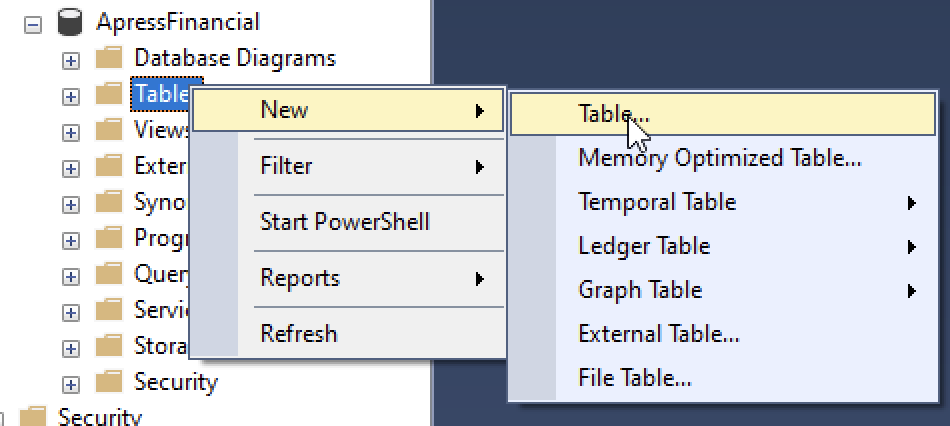
\includegraphics[width=0.7\textwidth]{images/task-1/1.png}
  \caption{Меню открытия конструктора таблиц}
  \label{fig:task-1-1}
\end{figure}

\begin{figure}[H]
  \centering
  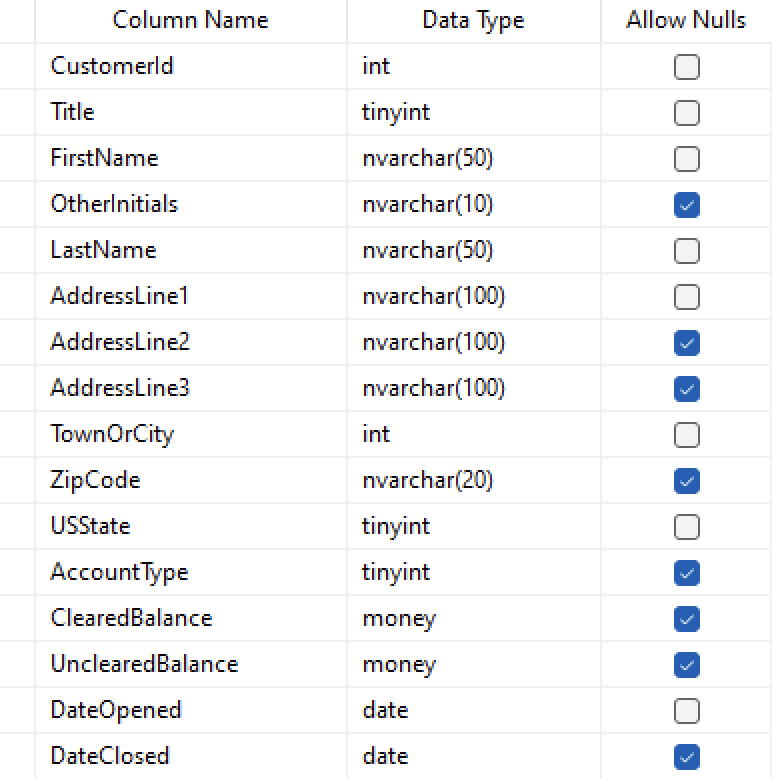
\includegraphics[width=0.7\textwidth]{images/task-1/2.png}
  \caption{Заполненные столбцы таблицы}
  \label{fig:task-1-2}
\end{figure}

\subsubsection{Настройка первичного ключа}

Для столбца <<CustomerId>> был настроен первичный ключ с помощью кнопки <<Set
Primary Key>> в контекстном меню, как это показано на рисунке
\ref{fig:task-1-3}.

\begin{figure}[H]
  \centering
  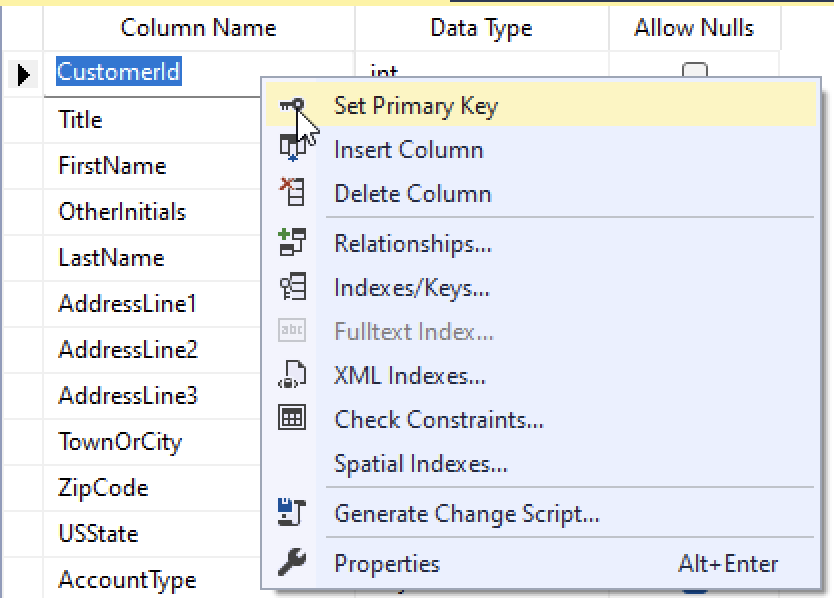
\includegraphics[width=0.7\textwidth]{images/task-1/3.png}
  \caption{Настройка первичного ключа}
  \label{fig:task-1-3}
\end{figure}

\subsubsection{Настройка индексов}

Для столбца <<CustomerId>> также был настроен индекс. С помощью кнопки
<<Indexes/Keys>> в контекстном меню, как показано на рисунке \ref{fig:task-1-4}.
В поле <<Name>> для индекса было указано имя <<PK\_Customers>>, а также
установлено свойство <<Create As Clustered>> в значение <<Yes>> (рисунок
\ref{fig:task-1-5}).

\begin{figure}[H]
  \centering
  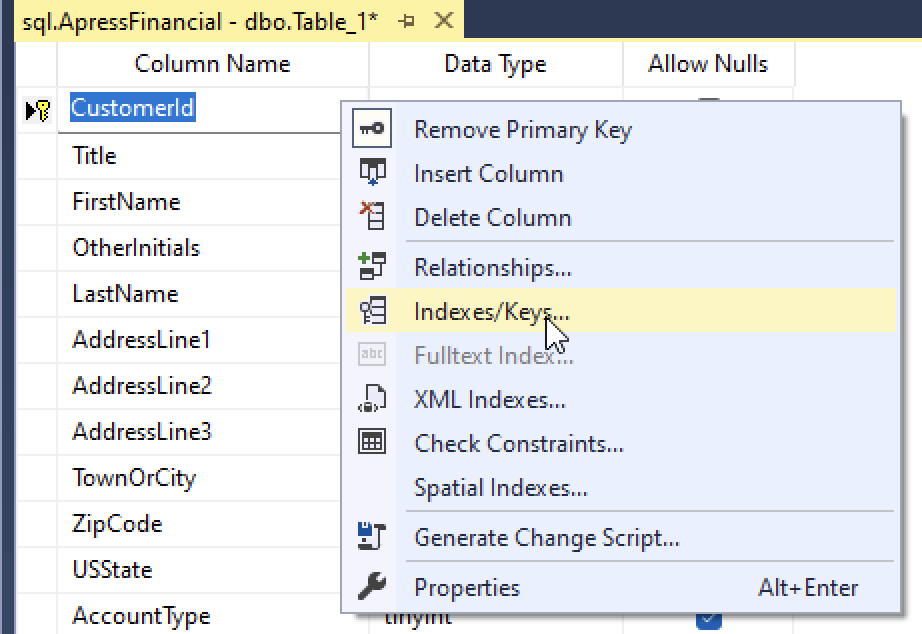
\includegraphics[width=0.7\textwidth]{images/task-1/4.png}
  \caption{Открытие настроек индексов}
  \label{fig:task-1-4}
\end{figure}

\begin{figure}[H]
  \centering
  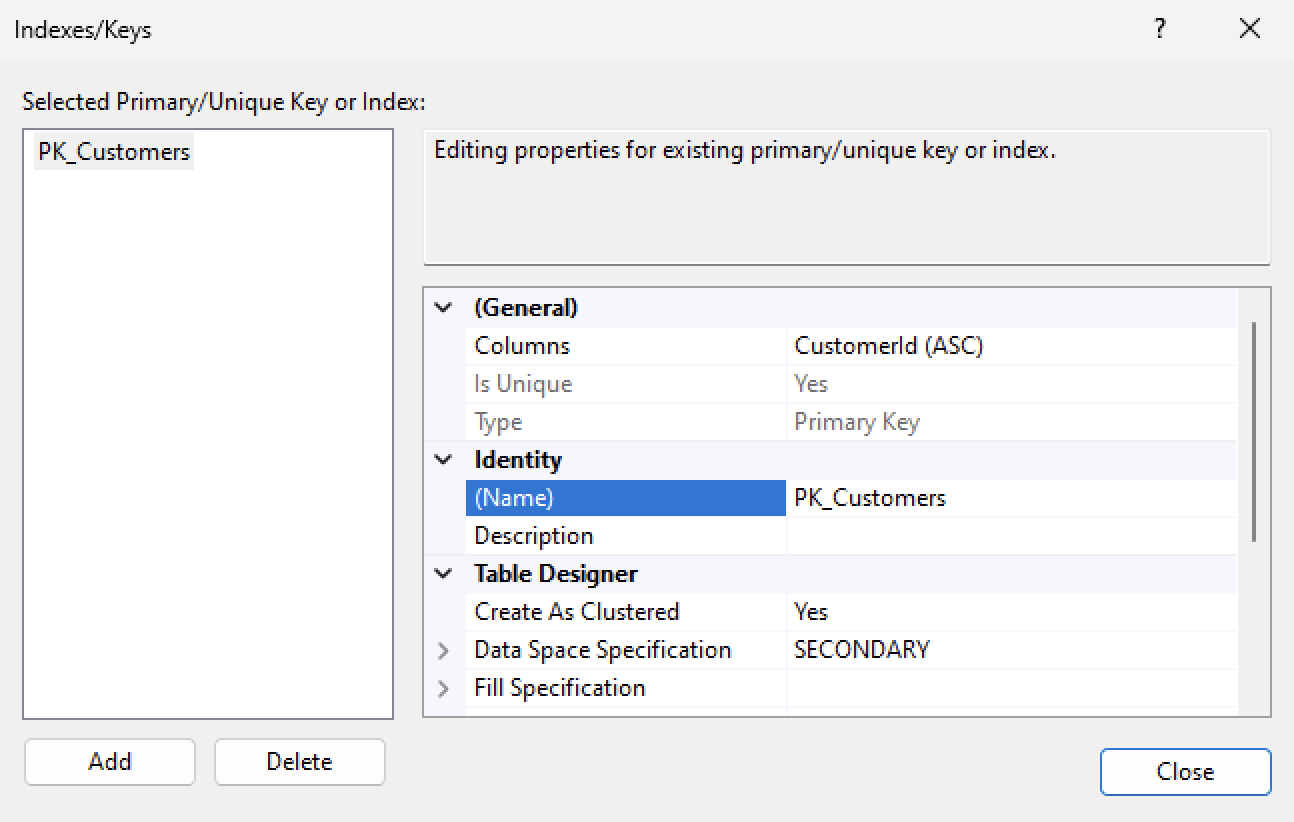
\includegraphics[width=\textwidth]{images/task-1/5.png}
  \caption{Настройка индексов}
  \label{fig:task-1-5}
\end{figure}

\subsubsection{Настройка столбцов}

В разделе <<Column Properties>>, как это показано на рисунке
\ref{fig:task-1-6}, для столбца <<CustomerId>> было установлено свойство <<IS
Identity>> в значение <<Yes>>. Для столбца <<DateOpened>> свойство <<Default
Value or Binding>> было установлено значение <<getdate()>>, что показано на
рисунке \ref{fig:task-1-7}.

\begin{figure}[H]
  \centering
  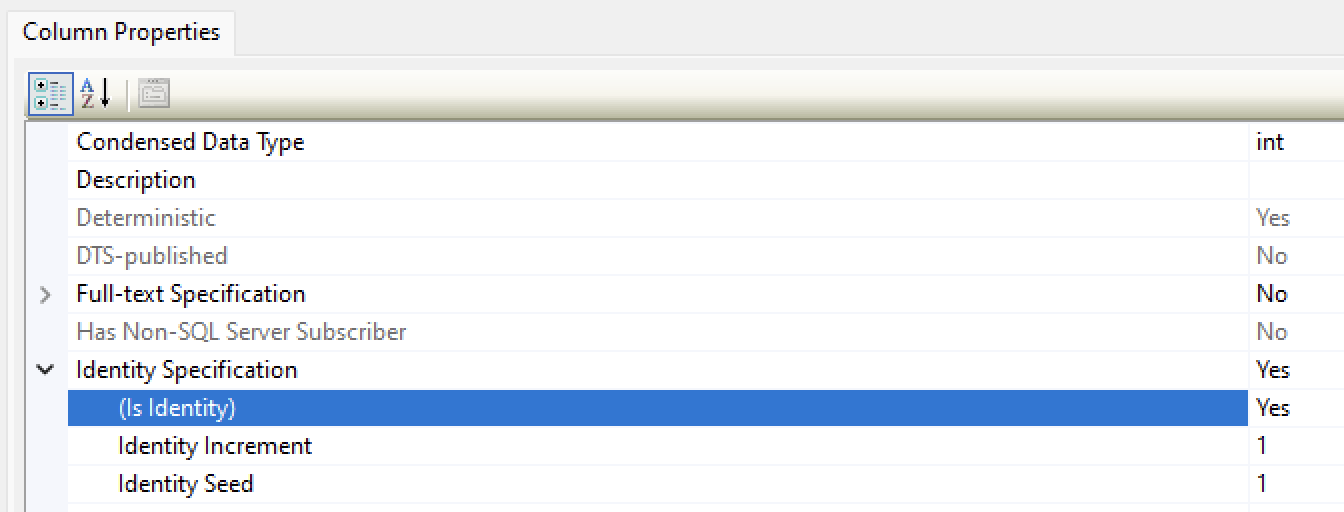
\includegraphics[width=\textwidth]{images/task-1/6.png}
  \caption{Настройка столбца CustomerId}
  \label{fig:task-1-6}
\end{figure}

\begin{figure}[H]
  \centering
  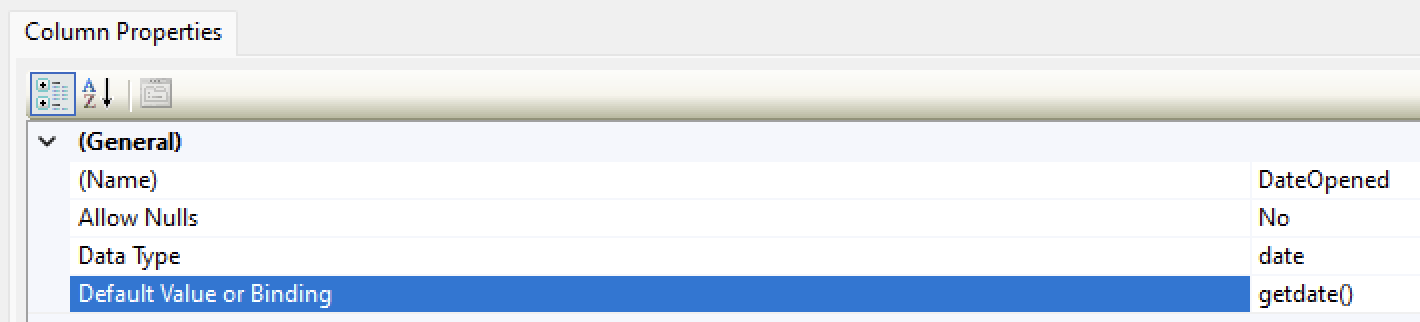
\includegraphics[width=0.8\textwidth]{images/task-1/7.png}
  \caption{Настройка столбца DateOpened}
  \label{fig:task-1-7}
\end{figure}

\subsubsection{Настройка свойств таблицы}

С помощью кнопки <<Properties Window>> на панели инструментов (рисунок
\ref{fig:task-1-8}) было открыто окно свойств таблицы. В нем для таблицы было
указано описание для создаваемой таблицы (рисунок \ref{fig:task-1-9}).

\begin{figure}[H]
  \centering
  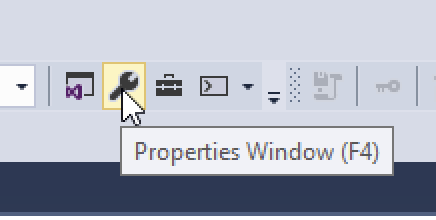
\includegraphics[width=0.4\textwidth]{images/task-1/8.png}
  \caption{Кнопка открытия свойств таблицы}
  \label{fig:task-1-8}
\end{figure}

\begin{figure}[H]
  \centering
  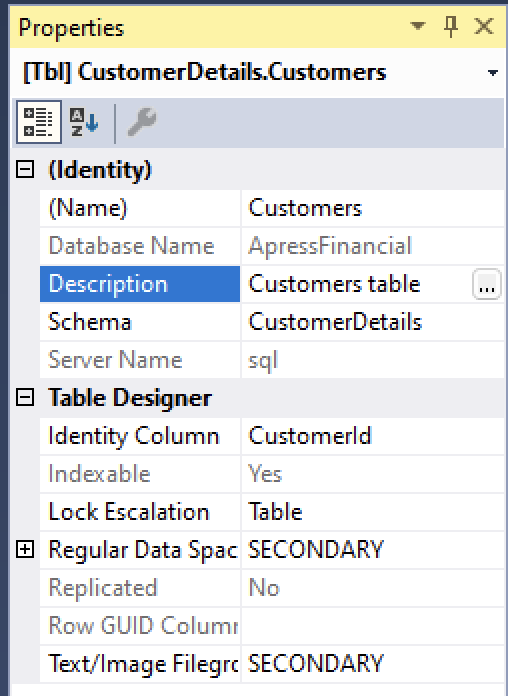
\includegraphics[width=0.4\textwidth]{images/task-1/9.png}
  \caption{Свойства таблицы}
  \label{fig:task-1-9}
\end{figure}

\subsubsection{Сохранение таблицы}

С помощью кнопки <<Save Customers>> на панели инструментов (рисунок
\ref{fig:task-1-10}) была сохранена таблица <<Customers>>. После этого она
появилась в интерфейсе SSMS.

\begin{figure}[H]
  \centering
  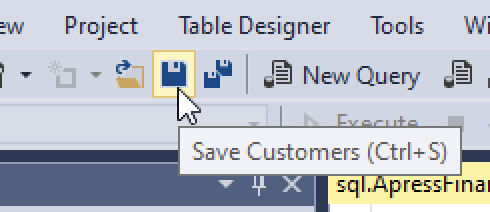
\includegraphics[width=0.5\textwidth]{images/task-1/10.png}
  \caption{Кнопка сохранения таблицы}
  \label{fig:task-1-10}
\end{figure}

\subsubsection{Просмотр свойств таблицы}

С помощью кнопки <<Properties>> в контекстном меню (рисунок \ref{fig:task-1-11})
были открыты свойства таблицы <<Customers>>. Они показаны на рисунке
\ref{fig:task-1-12}.

\begin{figure}[H]
  \centering
  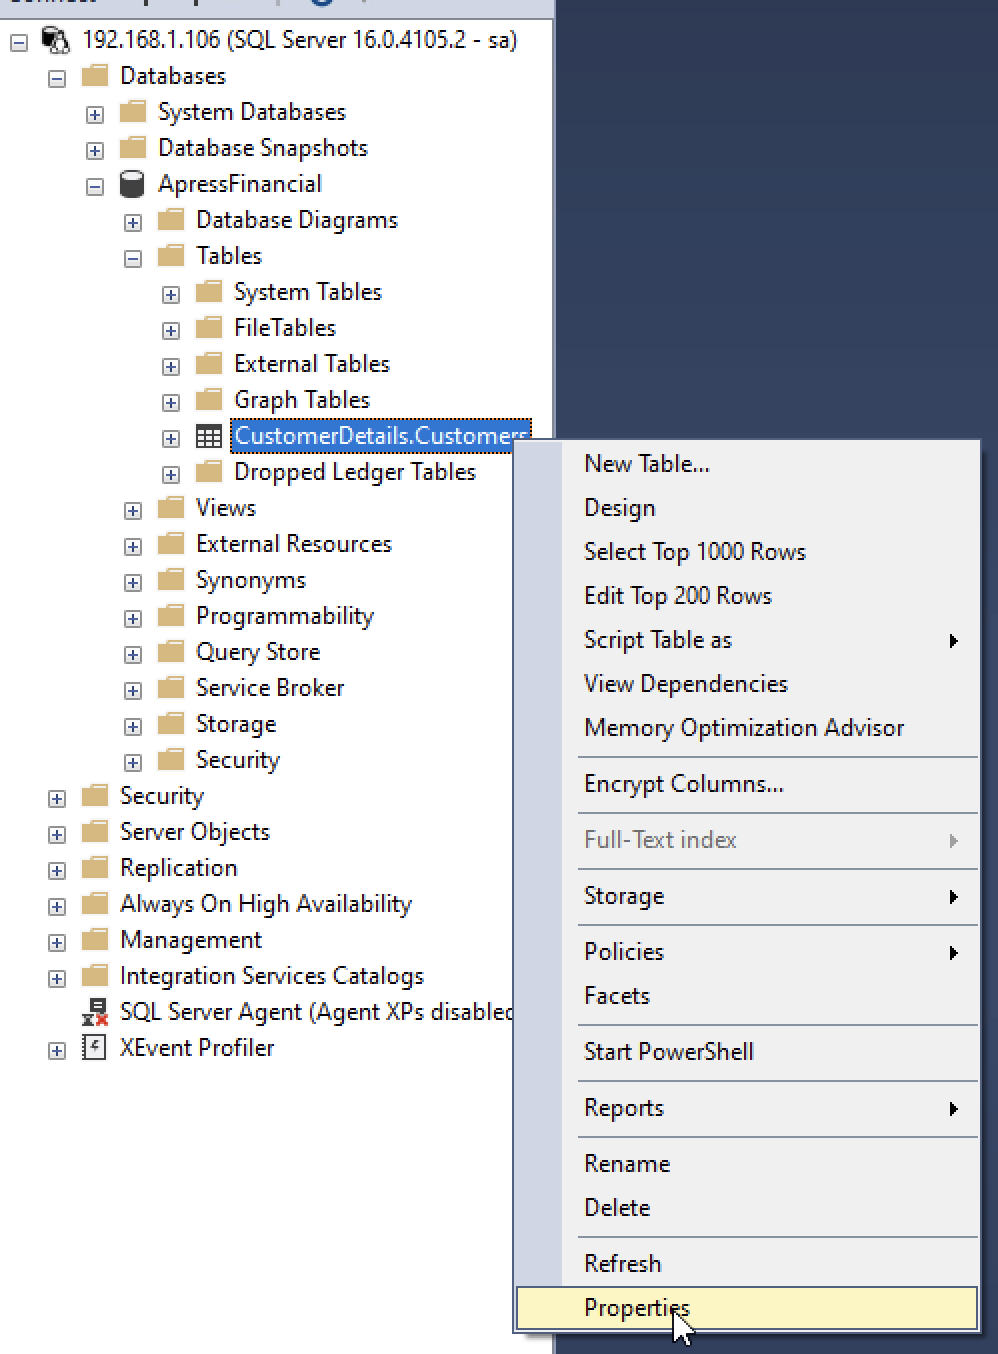
\includegraphics[width=0.5\textwidth]{images/task-1/11.png}
  \caption{Кнопка открытия свойств таблицы}
  \label{fig:task-1-11}
\end{figure}

\begin{figure}[H]
  \centering
  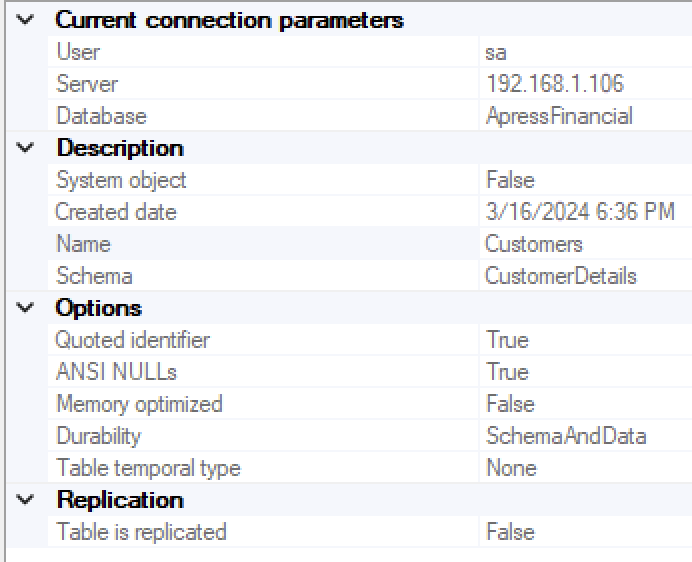
\includegraphics[width=0.7\textwidth]{images/task-1/12.png}
  \caption{Свойства таблицы <<Customers>>}
  \label{fig:task-1-12}
\end{figure}

\subsection{Вторая задача}

\subsubsection{Создание таблицы в Query Editor}

С помощью кнопки <<New Query>> на панели инструментов (рисунок
\ref{fig:task-2-1}) был открыт редактор запросов. В нем, в соответствии с
задании, был введен запрос, показанный на рисунке \ref{fig:task-2-2}. После
выполнения данного запроса в базе данных
<<\foreignlanguage{english}{ApressFinancial}>> была создана таблица
<<Transactions>> (рисунок \ref{fig:task-2-3}).

\begin{figure}[H]
  \centering
  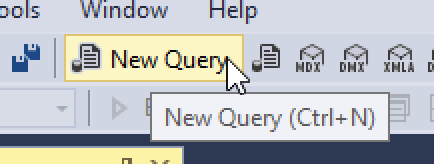
\includegraphics[width=0.5\textwidth]{images/task-2/1.png}
  \caption{Кнопка открытия редактора запросов}
  \label{fig:task-2-1}
\end{figure}

\begin{figure}[H]
  \centering
  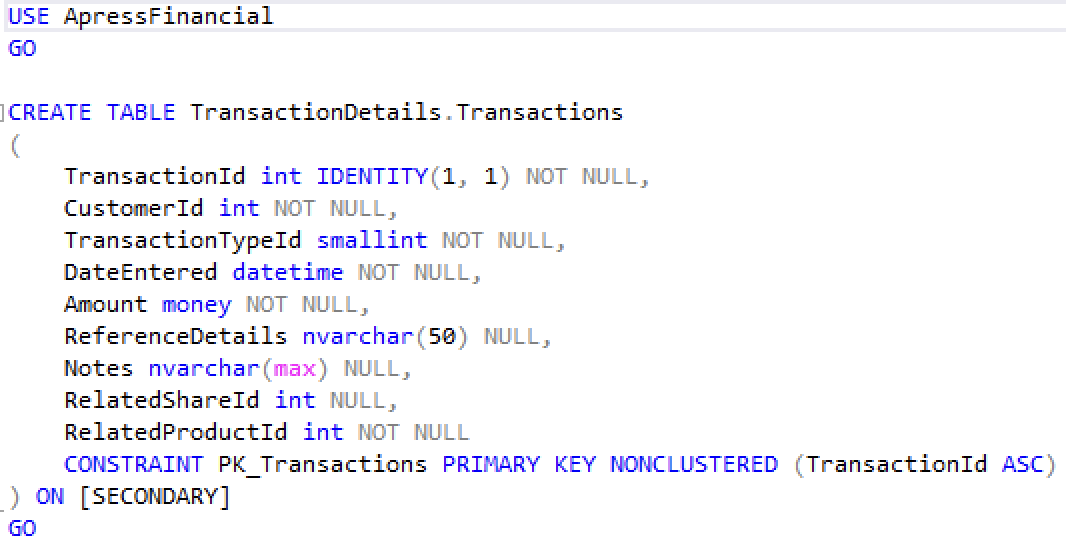
\includegraphics[width=\textwidth]{images/task-2/2.png}
  \caption{Запрос для создания таблицы <<Transactions>>}
  \label{fig:task-2-2}
\end{figure}

\begin{figure}[H]
  \centering
  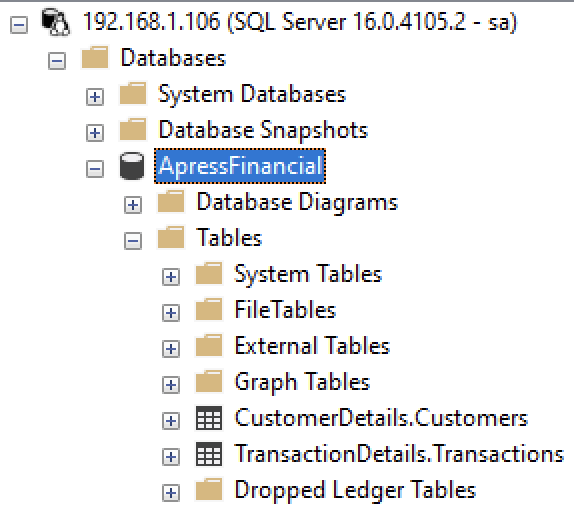
\includegraphics[width=0.5\textwidth]{images/task-2/3.png}
  \caption{Созданная таблица <<Transactions>>}
  \label{fig:task-2-3}
\end{figure}

\subsection{Третья задача}

\subsubsection{Генерация шаблона}

В обозревателе шаблонов был выбран шаблон <<Create Table>> (рисунок
\ref{fig:task-3-1}), после чего был сгенерирован запрос, показанный на рисунке
\ref{fig:task-3-2}.

\begin{figure}[H]
  \centering
  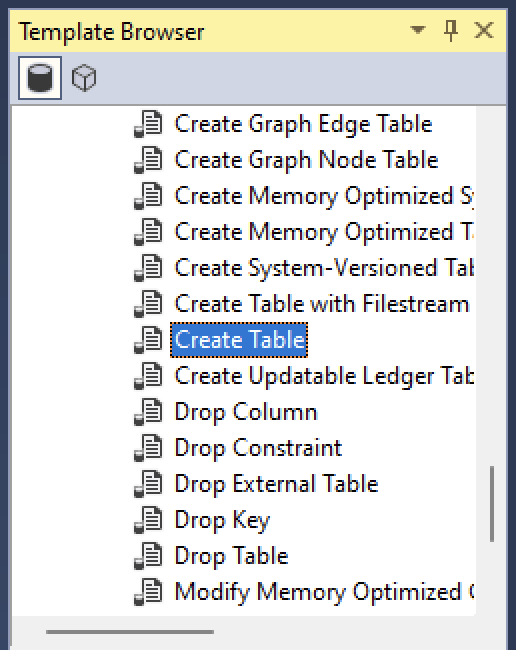
\includegraphics[width=0.5\textwidth]{images/task-3/1.png}
  \caption{Выбор шаблона}
  \label{fig:task-3-1}
\end{figure}

\begin{figure}[H]
  \centering
  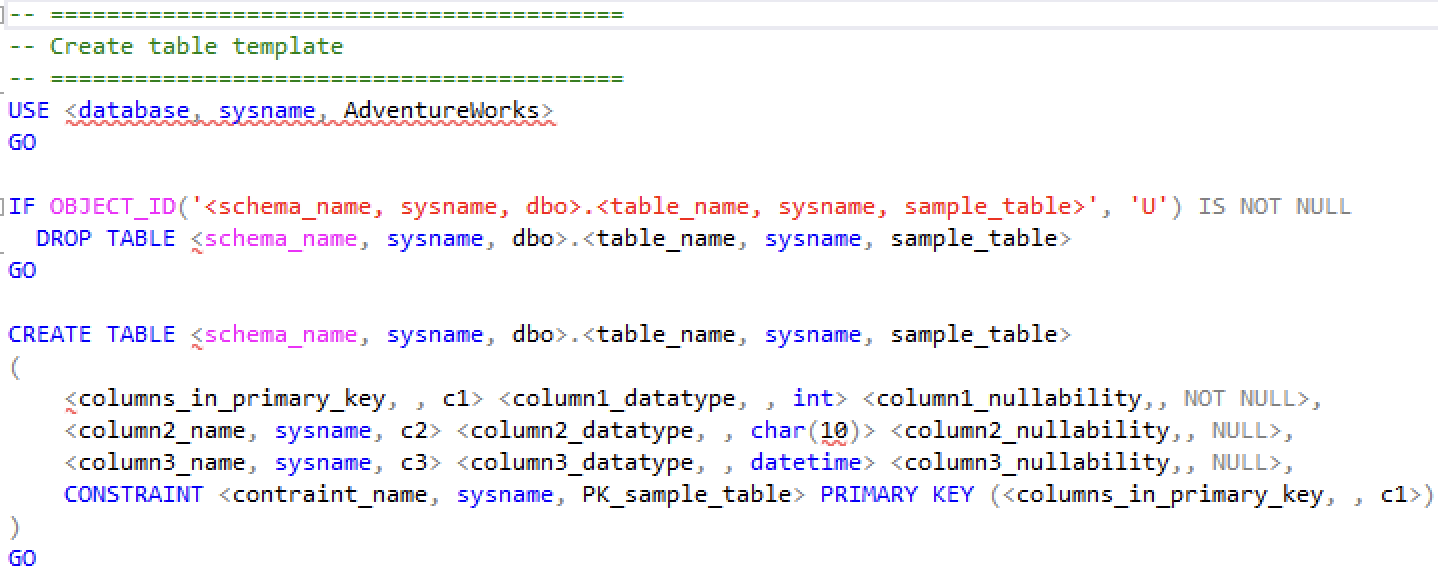
\includegraphics[width=\textwidth]{images/task-3/2.png}
  \caption{Результат генерации шаблона}
  \label{fig:task-3-2}
\end{figure}

\subsubsection{Изменение переменных шаблона}

Для изменения значения переменных шаблона на панели инструментов была нажата
кнопка, показанная на рисунке \ref{fig:task-3-3}. После этого было открыто окно,
в котором указываются значения переменных. В соответствии с заданием, были
указаны значения, показанные на рисунке \ref{fig:task-3-4}. После нажатия кнопки
<<ОК>> получился запрос, показанный на рисунке \ref{fig:task-3-5}.

\begin{figure}[H]
  \centering
  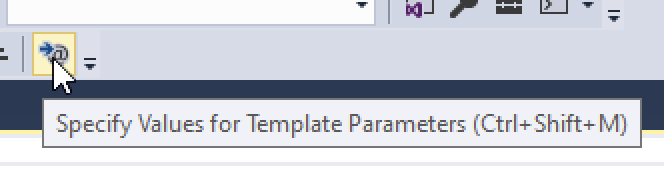
\includegraphics[width=0.7\textwidth]{images/task-3/3.png}
  \caption{Кнопка изменения переменных шаблона}
  \label{fig:task-3-3}
\end{figure}

\begin{figure}[H]
  \centering
  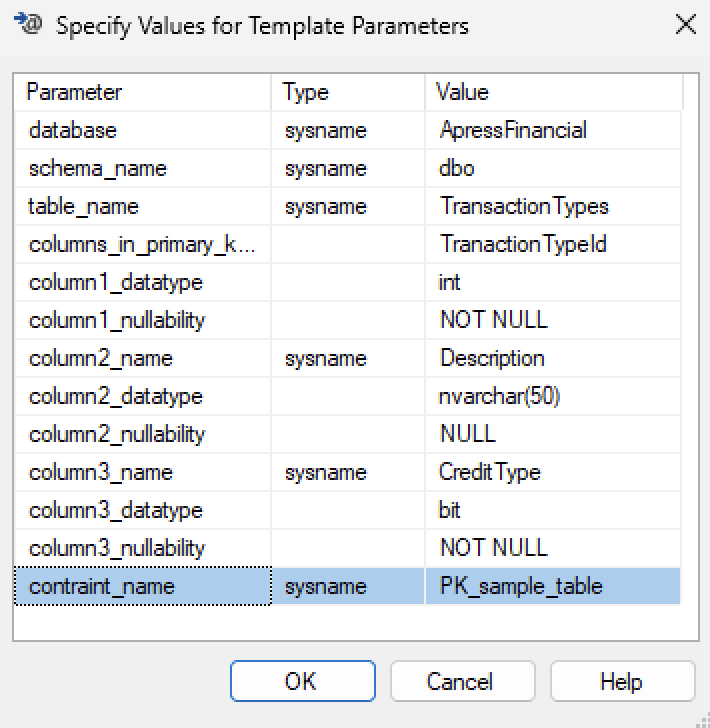
\includegraphics[width=0.7\textwidth]{images/task-3/4.png}
  \caption{Значения переменных шаблона}
  \label{fig:task-3-4}
\end{figure}

\begin{figure}[H]
  \centering
  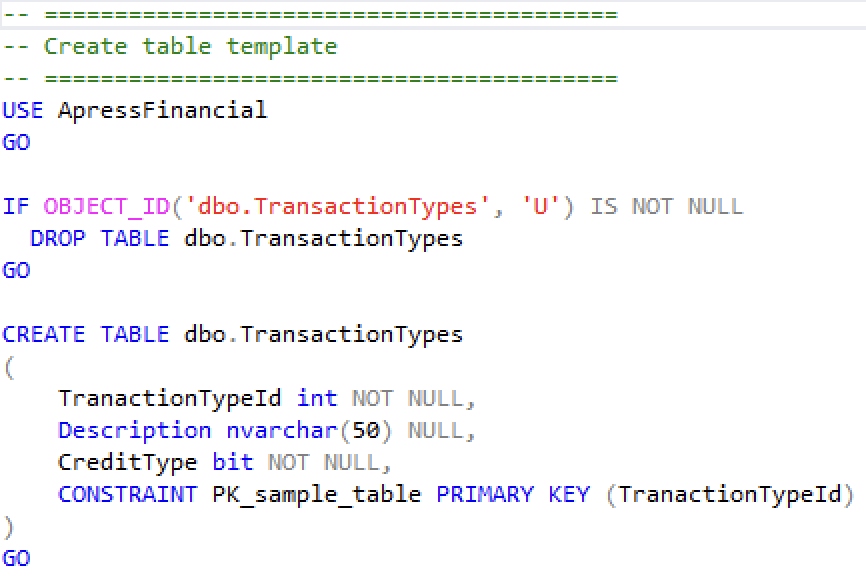
\includegraphics[width=\textwidth]{images/task-3/5.png}
  \caption{Получившийся запрос после изменения переменных}
  \label{fig:task-3-5}
\end{figure}

\subsubsection{Корректирование запроса}

В соответствии с заданием, запрос был скорректирован таким образом, как показано
на рисунке \ref{fig:task-3-6}. После его выполнения таблица появилась в
обозревателе SSMS (рисунок \ref{fig:task-3-7}).

\begin{figure}[H]
  \centering
  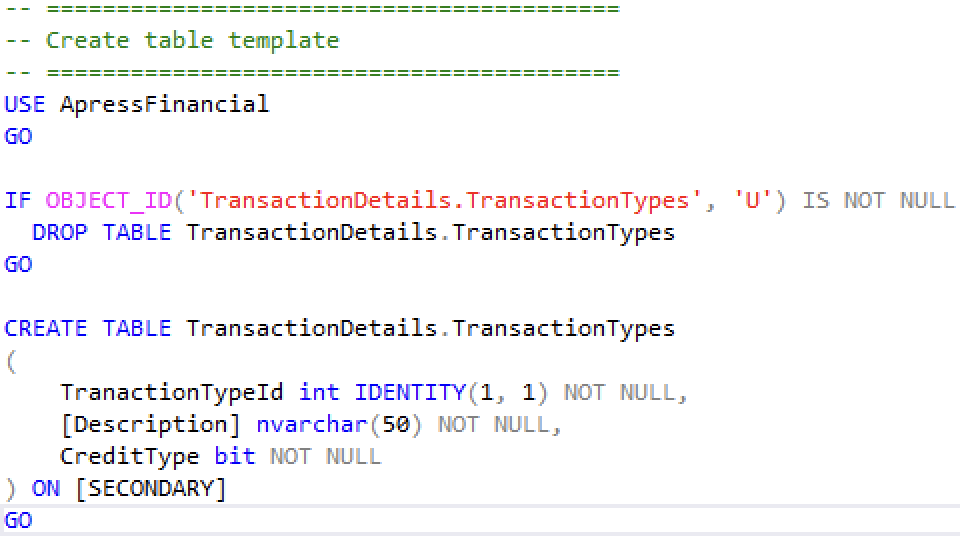
\includegraphics[width=\textwidth]{images/task-3/6.png}
  \caption{Итоговый запрос}
  \label{fig:task-3-6}
\end{figure}

\begin{figure}[H]
  \centering
  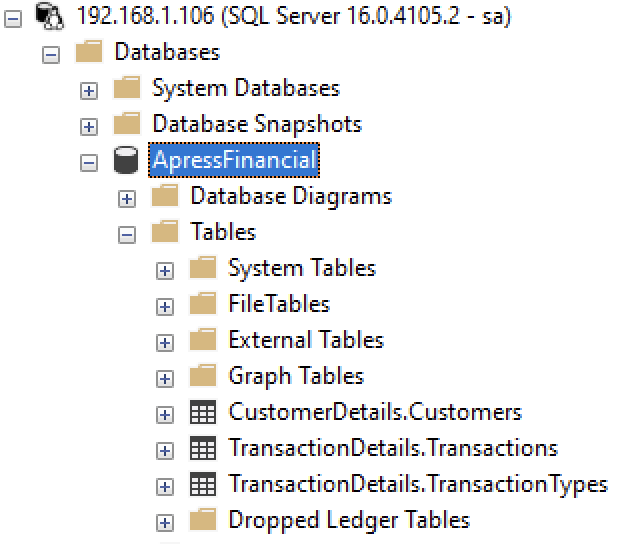
\includegraphics[width=0.5\textwidth]{images/task-3/7.png}
  \caption{Созданная таблица в SSMS}
  \label{fig:task-3-7}
\end{figure}

\subsection{Четвертая задача}

\subsubsection{Добавление столбца}

С помощью запроса, показанного на рисунке \ref{fig:task-4-1}, в таблицу
<<TransactionTypes>> был добавлен столбец <<AffectCashBalance>>.

\begin{figure}[H]
  \centering
  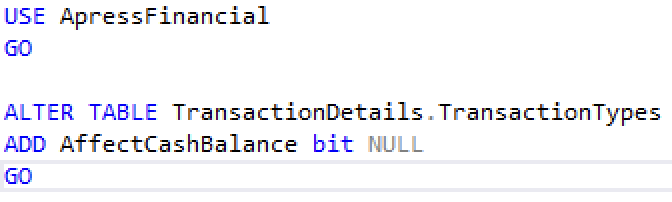
\includegraphics[width=0.8\textwidth]{images/task-4/1.png}
  \caption{Запрос на добавление столбца в таблицу}
  \label{fig:task-4-1}
\end{figure}

\subsubsection{Изменение столбца}

С помощью запроса, показанного на рисунке \ref{fig:task-4-2}, в таблице
<<TransactionTypes>> был изменен столбец <<AffectCashBalance>>: до этого столбец
был необязательным и мог хранить значение NULL, теперь столбец стал
обязательным.

\begin{figure}[H]
  \centering
  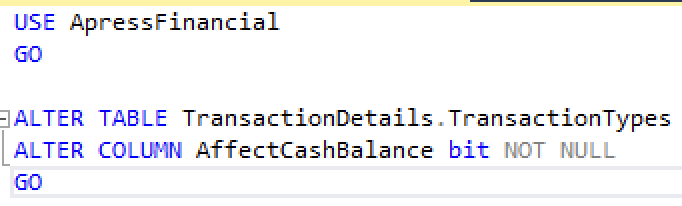
\includegraphics[width=0.8\textwidth]{images/task-4/2.png}
  \caption{Запрос на изменение столбца в таблице}
  \label{fig:task-4-2}
\end{figure}

\subsubsection{Добавление первичного ключа}

С помощью запроса, показанного на рисунке \ref{fig:task-4-3}, в таблицу
<<TransactionTypes>> был добавлен первичный ключ <<TransactionTypeId>>.

\begin{figure}[H]
  \centering
  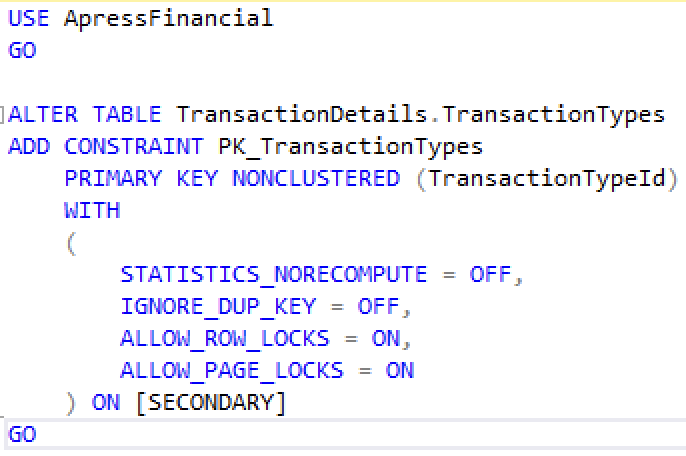
\includegraphics[width=0.8\textwidth]{images/task-4/3.png}
  \caption{Запрос на создание первичного ключа в таблице}
  \label{fig:task-4-3}
\end{figure}

\subsection{Пятая задача}

\subsubsection{Создание остальных таблиц}

В редакторе запросов был введен запрос, показанный на рисунке
\ref{fig:task-5-1}. Данный запрос создает таблицы <<FinancialProducts>>,
<<CustomerProducts>>, схему <<\foreignlanguage{english}{ShareDetails}>>, а также
таблицы <<Shares>> и <<SharePrices>>. После выполнения запроса данные таблицы
появились в SSMS (рисунок \ref{fig:task-5-2}).

\begin{figure}[H]
  \centering
  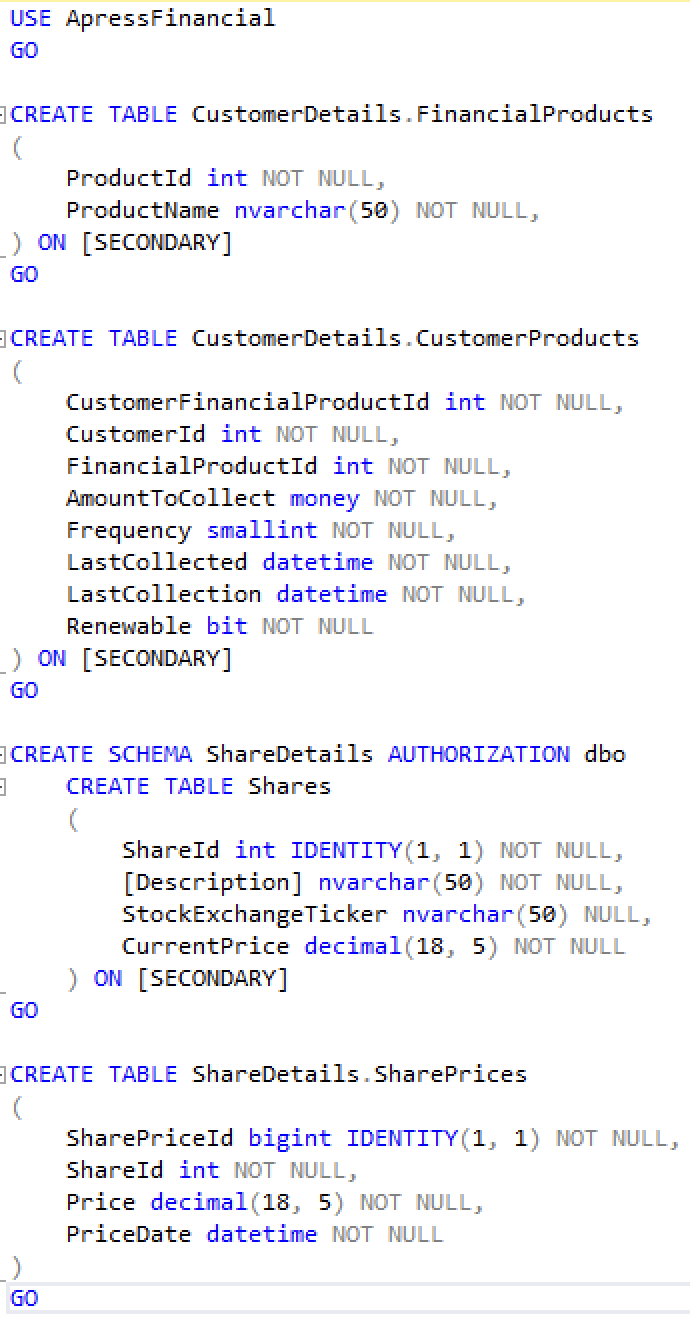
\includegraphics[width=0.7\textwidth]{images/task-5/1.png}
  \caption{Запрос для создания остальных таблиц}
  \label{fig:task-5-1}
\end{figure}

\begin{figure}[H]
  \centering
  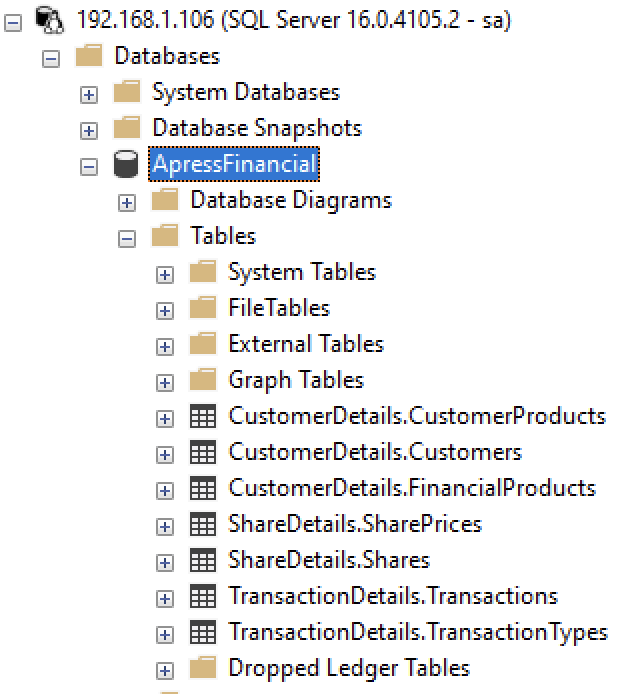
\includegraphics[width=0.5\textwidth]{images/task-5/2.png}
  \caption{Созданные таблицы в SSMS}
  \label{fig:task-5-2}
\end{figure}

\subsection{Шестая задача}

\subsubsection{Открытие редактора отношений}

С помощью кнопки <<Design>> в контекстном меню (рисунок \ref{fig:task-6-1}) был
открыт конструктор таблиц. В нем было открыто меню <<Relationships>> с помощью
кнопки в контекстном меню, показанном на рисунке \ref{fig:task-6-2}.

\begin{figure}[H]
  \centering
  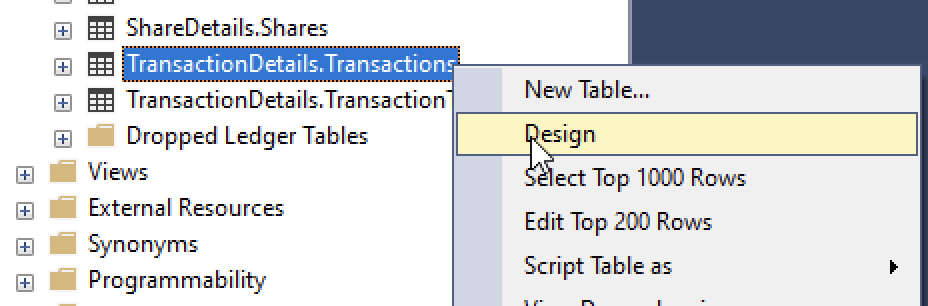
\includegraphics[width=0.7\textwidth]{images/task-6/1.png}
  \caption{Кнопка открытия конструктора таблиц}
  \label{fig:task-6-1}
\end{figure}

\begin{figure}[H]
  \centering
  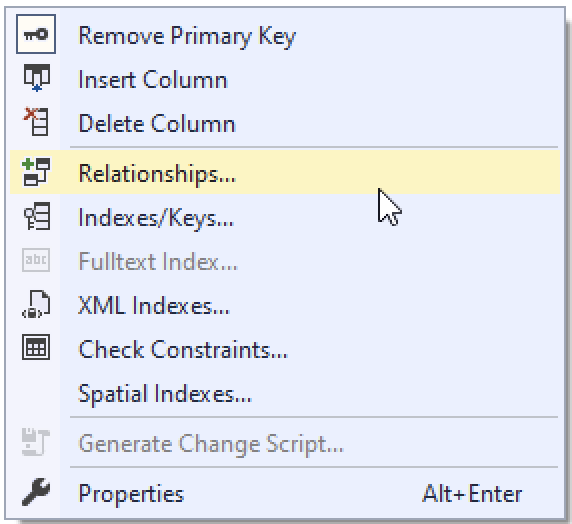
\includegraphics[width=0.5\textwidth]{images/task-6/2.png}
  \caption{Кнопка открытия окна отношений}
  \label{fig:task-6-2}
\end{figure}

\subsubsection{Создание связи}

В редакторе отношений с помощью кнопки, показанной на рисунке
\ref{fig:task-6-3}, было открыто окно создания новой связи. В нем было изменено
значение поля <<\foreignlanguage{english}{Relationship Name}>> на
<<FK\_Transactions\_Customers>> (рисунок \ref{fig:task-6-4}). В поле <<Primary
key Table>> была выбрана таблица <<Customers>>, а в поле <<Foreign key Table>>
был выбран столбец <<CustomerId>> (рисунок \ref{fig:task-6-5}). После нажатия на
кнопку <<ОК>> и сохранения изменений в SSMS появилась связь между таблицами.

\begin{figure}[H]
  \centering
  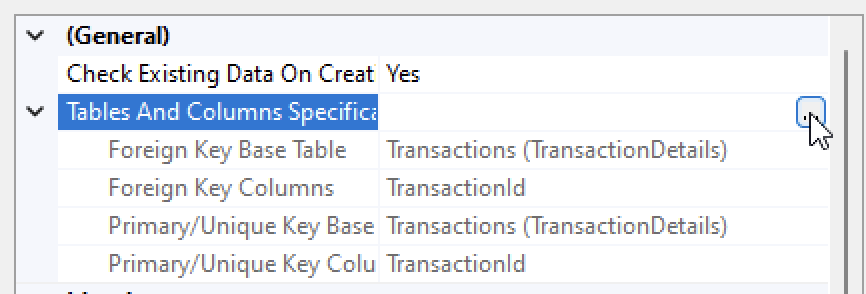
\includegraphics[width=0.8\textwidth]{images/task-6/3.png}
  \caption{Кнопка создания новой связи}
  \label{fig:task-6-3}
\end{figure}

\begin{figure}[H]
  \centering
  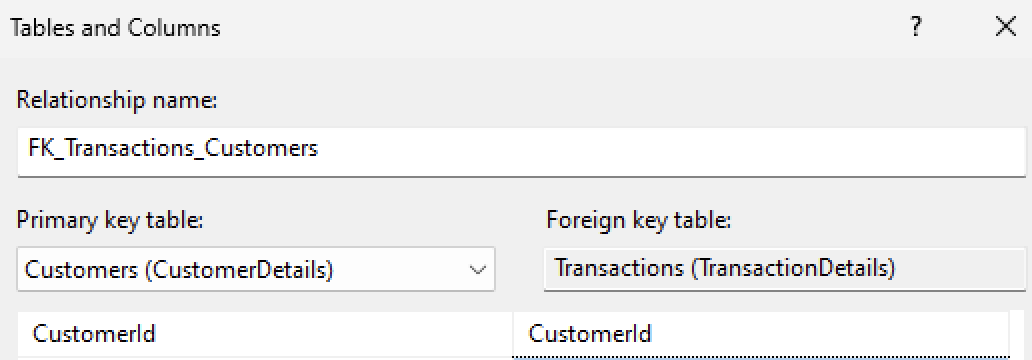
\includegraphics[width=0.8\textwidth]{images/task-6/4.png}
  \caption{Поле для ввода <<Relationship Name>>}
  \label{fig:task-6-4}
\end{figure}

\begin{figure}[H]
  \centering
  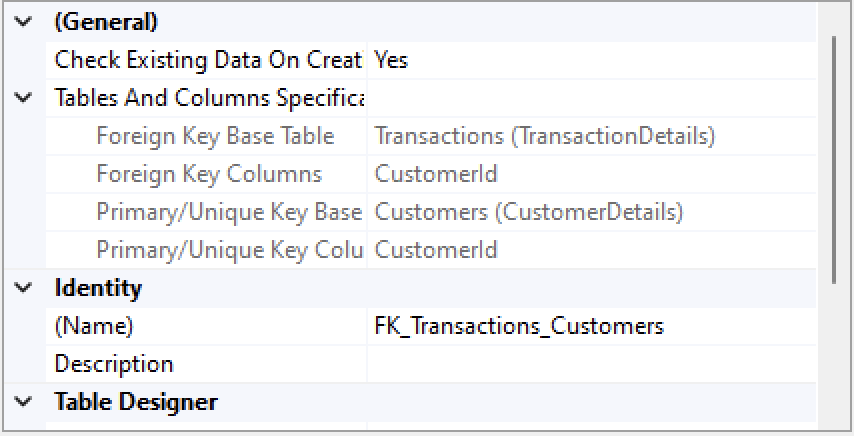
\includegraphics[width=0.8\textwidth]{images/task-6/5.png}
  \caption{Поля для выбора столбцов}
  \label{fig:task-6-5}
\end{figure}

\subsection{Седьмая задача}

\subsubsection{Создание связи}

С помощью запроса, показанного на рисунке \ref{fig:task-7-1}, создается связь
между таблицам <<Transactions>> и <<Shares>>. Однако при выполнении этого запроса
возникает ошибка, показанная на рисунке \ref{fig:task-7-2}. Это происходит
потому, что в таблице <<Shares>> отсутствует первичный ключ <<ShareId>>.

\begin{figure}[H]
  \centering
  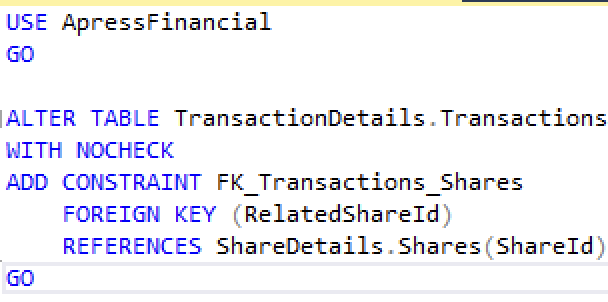
\includegraphics[width=0.6\textwidth]{images/task-7/1.png}
  \caption{Запрос для создания связи}
  \label{fig:task-7-1}
\end{figure}

\begin{figure}[H]
  \centering
  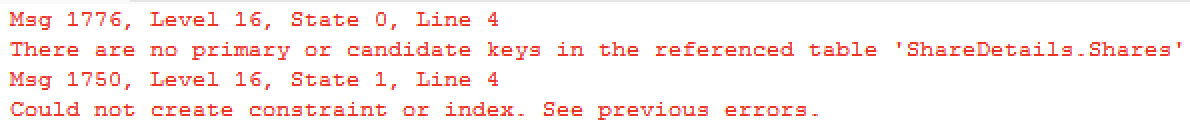
\includegraphics[width=\textwidth]{images/task-7/2.png}
  \caption{Ошибка, возникшая при выполнении запроса}
  \label{fig:task-7-2}
\end{figure}

\subsubsection{Устранение ошибки}

Для устранения ошибки, описанной выше, был выполнен запрос, показанный на
рисунке \ref{fig:task-7-3}. Данный запрос добавляет отсутствующий первичный ключ
в таблицу <<ShareId>>. После выполнения данного запроса, запрос, показанный на
рисунке \ref{fig:task-7-1}, был успешно выполнен и связь была создана.

\begin{figure}[H]
  \centering
  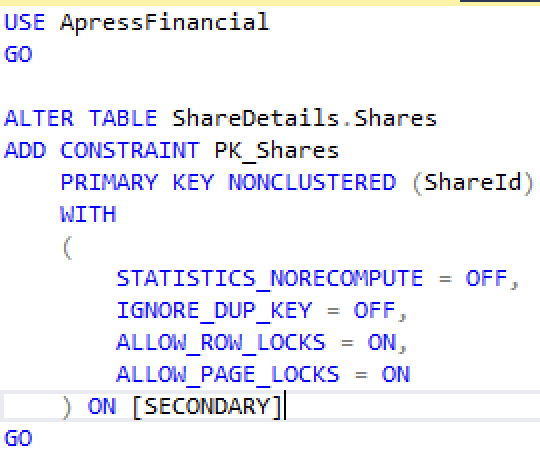
\includegraphics[width=0.5\textwidth]{images/task-7/3.png}
  \caption{Запрос для создания первичного ключа}
  \label{fig:task-7-3}
\end{figure}

\section{Выводы и анализ результатов работы}

В данной лабораторной работе изучены способы создания таблиц с помощью
конструктора таблиц SSMS и с помощью запросов на языке T-SQL, а также способы
добавления и изменения столбцов.

Цель, поставленная в начале работы, достигнута, задачи выполнены.

\end{document}
